\documentclass[final]{beamer}
\usepackage{algorithmic}
\usepackage{algorithm}
\usepackage[orientation=portrait,
		size=custom, width=55.8, height=91.4,  % poster size 22in=55.88cm 91.44cm=36in
		scale=.99
	]{beamerposter}
\usepackage{listings}
\usepackage[american]{babel}  % language 
\usepackage[utf8]{inputenc}   % std linux encoding

\usetheme{pgassc11poster}            % our poster style
%--set colors for blocks (without frame)---------------------------------------
\setbeamercolor{block title}{fg=ngreen,bg=white}
\setbeamercolor{block body}{fg=black,bg=white}
%--set colors for alerted blocks (with frame)----------------------------------
%--textcolor = fg, backgroundcolor = bg, dblue is the jacobs blue
\setbeamercolor{block alerted title}{fg=white,bg=dblue!70}%frame color
\setbeamercolor{block alerted body}{fg=black,bg=dblue!10}%body color

%==Titel, date and authors of the poster=======================================
\title{Alternative High Performance Benchmarks}
\author{Kurt Rudolph, Vivek Kale, Lawrence C. Angrave, William D. Gropp}
\institute{Department of Computer Science, University of Illinois Urbana-Champaign}
\date{\today}
%
%==some usefull qm commands====================================================
%  |x>
\newcommand{\ket}[1]{\left\vert#1\right\rangle}
%  <x|
\newcommand{\bra}[1]{\left\langle#1\right\vert}
%  <x|y>
\newcommand{\braket}[2]{\left< #1 \vphantom{#2}\, \right\vert\left.\!\vphantom{#1} #2 \right>}
%  <x|a|y>
\newcommand{\sandwich}[3]{\left< #1 \vphantom{#2 #3} \right #2 \left|\vphantom{#1 #2} #3 \right>}
%  d/dt
\newcommand{\ddt}{\frac{d}{dt}}
%  D/Dx
\newcommand{\pdd}[1]{\frac{\partial}{\partial#1}}
%  |x|
\newcommand{\abs}[1]{\left\vert#1\right\vert}
%  k_{x}
\newcommand{\kv}[1]{\mathbf{k}_{#1}}




\begin{document}
	\begin{frame}[t]
		\begin{columns}[t] 
			  \begin{column}{0.60\paperwidth} 
%=======================Avstract======================================================================================
				\begin{alertblock}{Abstract}
					Benchmarks for High-Performance clusters generally focus on floating-point intensive calculations. Few of these address data intensive graph operations, a class of computation rapidly growing in demand.  As an alternative to standard floating-point benchmarks, a new benchmark, the Graph 500 has been proposed. The benchmark employ's multiple implementations with the intention to identify desecrate performance aspects via the comparative results, however a PGAS model has yet to be developed. This project focuses on understanding what capabilities a UPC Graph 500 implementation may offer. Specifically: 1. the UPC expressibility for irregular graph operations of Graph 500 and 2. simple performance testing of the efficiency of UPC.
				\end{alertblock}
%=======================Linked List Traversal======================================================================================
				\begin{block}{Random Access}
					When performing graph operations, random access to memory and random process communication are generally very common.  This test looks at how well a UPC Graph 500 implementation of may handle these operations.  To do so, we implement a dot product employing randomized access and communication through the RDMA.   The affinity to the vectors are distributed across all processes in the group and colored according.  Successive vector positions are stored successive memory locations of the according process.  
				\end{block}
				\begin{columns}[t,totalwidth=0.60\paperwidth]
					\begin{column}{0.28\paperwidth}
						\lstinputlisting[language=C, basicstyle=\footnotesize]{ code_sample/upcRandomAccess.c}
					\end{column}
					\begin{column}{0.28\paperwidth}
						\begin{columns}[t,totalwidth=0.28\paperwidth]
							\begin{column}{0.12\paperwidth}
								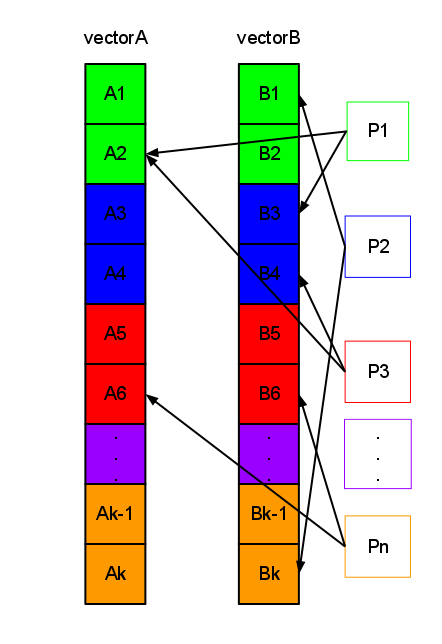
\includegraphics[width=0.12\paperwidth]{img/rand_access}
							\end{column}
							\begin{column}{0.12\paperwidth}
								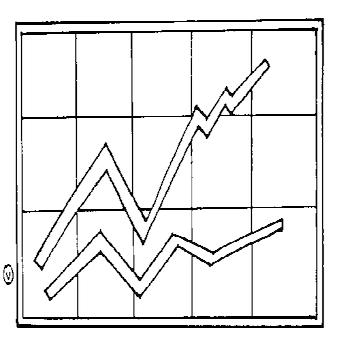
\includegraphics[width=0.12\paperwidth]{img/temp}
							\end{column}
						\end{columns}
					\end{column}
				\end{columns}
				\vskip1ex
%A UPC thread t_i first chooses a random cell in v1 that belongs to it:   v1[rand()%n];   
%A UPC thread t_i then chooses a random cell in v2 to multiply with:    v2[rand()%n];  

%There is 1/p chance that a thread will access its own partition. There is (p-1)/p chance that a thread will have to go through the RDMA to retrieve the data it needs to do the floating-point multiplication.

%Other variants exist:  

%  - each thread runs through its own partition v1[(n/p)*i]  to v1[(n/p)*i] ,  and for each choose  v2[rand()%(n/p) + (n/p)*i] based on thread partition each thread has.

 %  - each thread chooses a random cell in its partition  of v1  and then chooses a cell in its partition of v2. 
  
 % - choose whether you want to have distinct pairs, or have some cells  repeated across pairs, or entire pairs repeated. 


%These tests can be representative of graph traversal operations and irregular algorithms. They particularly test the class of computation UPC one-sided programming model would be used for. 
%=======================Linked List Traversal======================================================================================
				\begin{block}{Linked List Traversal}
					As a simple test to measure the efficiency of UPC when performing graph operations, various linked list structure have been built and a timed traversal is taken for each.  Similar to the previous test test, the affinity of the nodes are distributed across all processes in the group and colored according.  Successive nodes are stored in successive memory locations of the according process as well.  
				\end{block}
				\begin{columns}[t,totalwidth=0.60\paperwidth]
					\begin{column}{0.28\paperwidth}
						\begin{center} \bf{Sequential Node, Sequential Process} \end{center}
						\begin{columns}[t,totalwidth=0.28\paperwidth]
							\begin{column}{0.12\paperwidth}
								\begin{center} 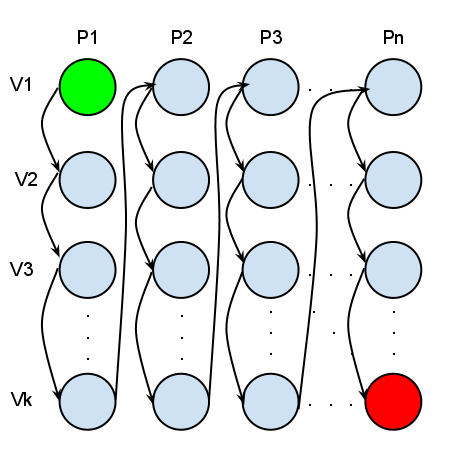
\includegraphics[width=0.12\paperwidth]{img/linked_list/seq_node_seq_proc} \end{center}
							\end{column}
							\begin{column}{0.12\paperwidth}
								\begin{center} 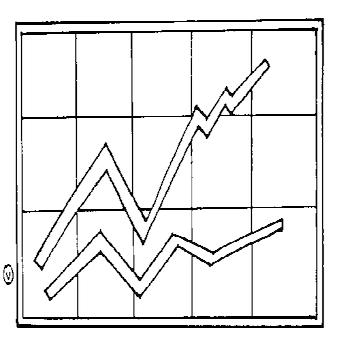
\includegraphics[width=0.12\paperwidth]{img/temp} \end{center}
							\end{column}
						\end{columns}
					\end{column}
					\begin{column}{0.28\paperwidth}
						\begin{center} \bf{Sequential Process, Sequential Node} \end{center}
						\begin{columns}[t,totalwidth=0.28\paperwidth]
							\begin{column}{0.12\paperwidth}
								\begin{center} 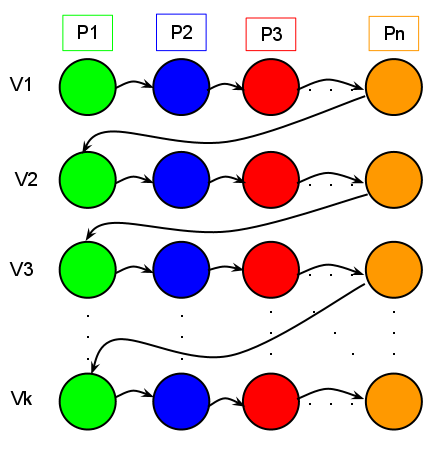
\includegraphics[width=0.12\paperwidth]{img/linked_list/seq_proc_seq_node} \end{center}
							\end{column}
							\begin{column}{0.12\paperwidth}
								\begin{center} 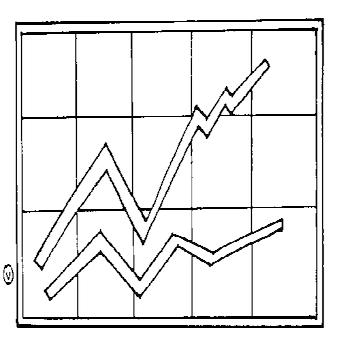
\includegraphics[width=0.12\paperwidth]{img/temp} \end{center}
							\end{column}
						\end{columns}
					\end{column}
				\end{columns}
				\begin{columns}[t,totalwidth=0.60\paperwidth]
					\begin{column}{0.28\paperwidth}
						\begin{center} \bf{Random Node, Sequential Process} \end{center}
						\begin{columns}[t,totalwidth=0.28\paperwidth]
							\begin{column}{0.12\paperwidth}
								\begin{center} 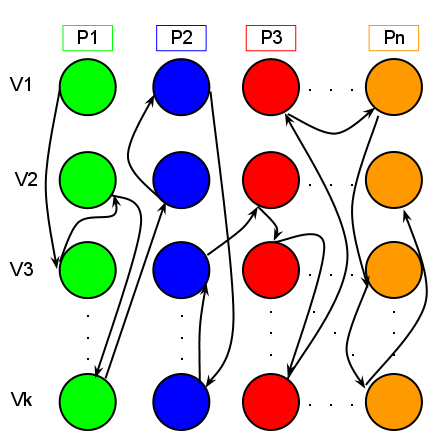
\includegraphics[width=0.12\paperwidth]{img/linked_list/rand_node_seq_proc} \end{center}
							\end{column}
							\begin{column}{0.12\paperwidth}
								\begin{center} 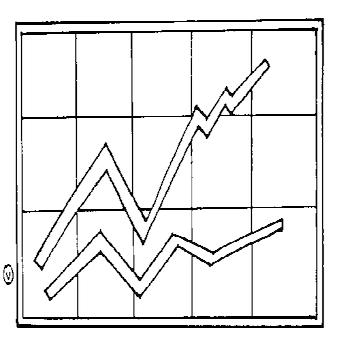
\includegraphics[width=0.12\paperwidth]{img/temp} \end{center}
							\end{column}
						\end{columns}
					\end{column}
					\begin{column}{0.28\paperwidth}
						\begin{center} \bf{Sequential Process, Random Node} \end{center}
						\begin{columns}[t,totalwidth=0.28\paperwidth]
							\begin{column}{0.12\paperwidth}
								\begin{center} 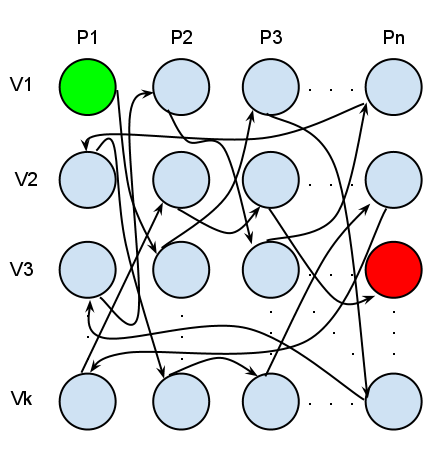
\includegraphics[width=0.12\paperwidth]{img/linked_list/seq_proc_rand_node} \end{center}
							\end{column}
							\begin{column}{0.12\paperwidth}
								\begin{center} 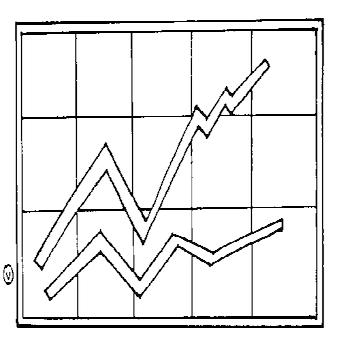
\includegraphics[width=0.12\paperwidth]{img/temp} \end{center}
							\end{column}
						\end{columns}
					\end{column}
				\end{columns}
				\begin{columns}[t,totalwidth=0.60\paperwidth]
					\begin{column}{0.28\paperwidth}
						\begin{center} \bf{Sequential Node, Random Process} \end{center}
						\begin{columns}[t,totalwidth=0.28\paperwidth]
							\begin{column}{0.12\paperwidth}
								\begin{center} 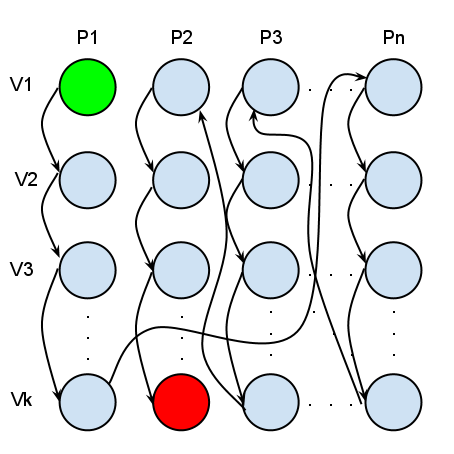
\includegraphics[width=0.12\paperwidth]{img/linked_list/seq_node_rand_proc} \end{center}
							\end{column}
							\begin{column}{0.12\paperwidth}
								\begin{center} 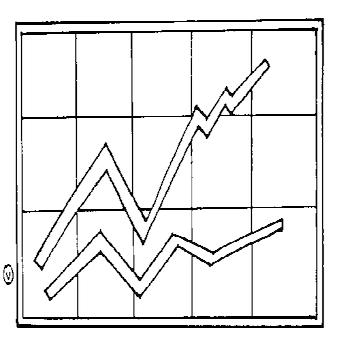
\includegraphics[width=0.12\paperwidth]{img/temp} \end{center}
							\end{column}
						\end{columns}
					\end{column}
					\begin{column}{0.28\paperwidth}
						\begin{center} \bf{Random Process, Sequential Node} \end{center}
						\begin{columns}[t,totalwidth=0.28\paperwidth]
							\begin{column}{0.12\paperwidth}
								\begin{center} 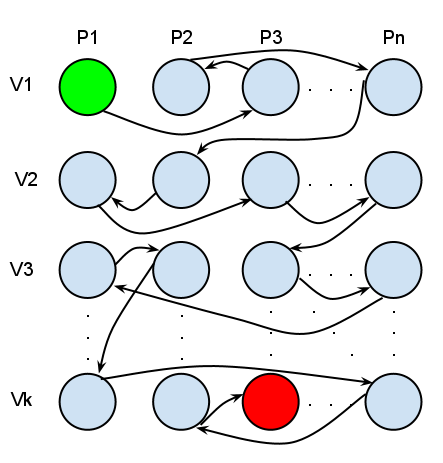
\includegraphics[width=0.12\paperwidth]{img/linked_list/rand_proc_seq_node} \end{center}
							\end{column}
							\begin{column}{0.12\paperwidth}
								\begin{center} 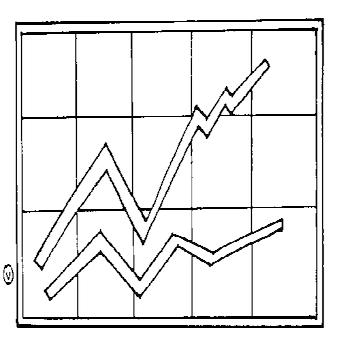
\includegraphics[width=0.12\paperwidth]{img/temp} \end{center}
							\end{column}
						\end{columns}
					\end{column}
				\end{columns}
				\begin{columns}[t,totalwidth=0.60\paperwidth]
					\begin{column}{0.28\paperwidth}
						\begin{center} \bf{Random Node, Random Process} \end{center}
						\begin{columns}[t,totalwidth=0.28\paperwidth]
							\begin{column}{0.12\paperwidth}
								\begin{center} 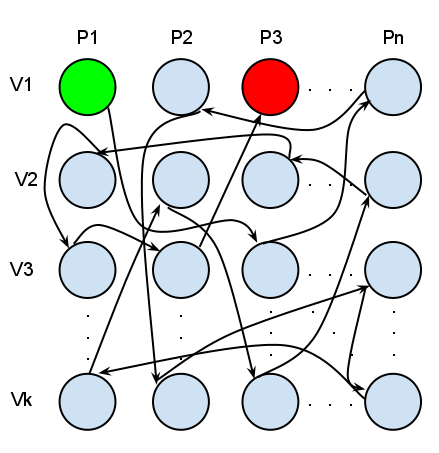
\includegraphics[width=0.12\paperwidth]{img/linked_list/rand_proc_rand_node} \end{center}
							\end{column}
							\begin{column}{0.12\paperwidth}
								\begin{center} 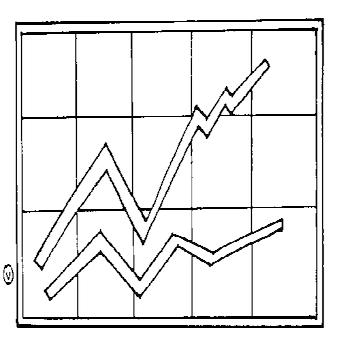
\includegraphics[width=0.12\paperwidth]{img/temp} \end{center}
							\end{column}
						\end{columns}
					\end{column}
					\begin{column}{0.28\paperwidth}
						Discussion of the results...........................................................
					\end{column}
				\end{columns}
%=======================Multi Process Linked List Traversal======================================================================================
			\end{column}
			\begin{column}{0.28\paperwidth}
%=======================Discussion=======================================================================================================
				\begin{block}{Graph 500 BFS}
				The Graph 500 currently employs multiple implementations using MPI and OpenMP.  
					
					The "Simple" MPI implementation achieves two-sided communication through communicator functions such as  \emph{send} and \emph{receive}. Sample from Graph500 BFS MPI Simple:\vspace{2 mm}
					\lstinputlisting[language=C, basicstyle=\footnotesize]{ code_sample/mpiSimpleSample.c}
					 \vspace{5 mm}
					  The "One Sided" MPI implementation achieves one-sided communication through MPI \emph{windows}, a feature built into MPICH2 API.  When a thread creates an MPI \emph{window} access to another threads address space is enabled through the variables associated through that window.  Sample from the Graph500 BFS MPI One Sided: 
					  \vspace{2 mm}
					  \lstinputlisting[language=C, basicstyle=\footnotesize]{ code_sample/mpiOneSidedSample.c} 
					  \vspace{5 mm}
					  A UPC implementation of the Graph 500 will not require "windows" to achieve one sided communication.  However, address space used in any collective operations need to be allocated in shared memory space and receive the according performance loss of accessing memory a shared pointer over a local pointer.  MPI collectives from the Graph500 BFS implemented in UPC take the simpler implementation as follows: 
					  \vspace{2 mm}
					  \lstinputlisting[language=C, basicstyle=\footnotesize]{ code_sample/upcOneSidedSample.c} 
				\end{block}
%=======================Conclusion========================================================================================================
				\begin{block}{Conclusion}
				\end{block}
%=======================References========================================================================================================
				\begin{block}{References}
					\begin{thebibliography}{7}
						{\small
						\bibitem{UPC_Language_Spcification}
							\url{http://upc.gwu.edu/docs/upc_specs_1.2.pdf}
						\bibitem{Introduction_To_UPC}
							  \url{http://upc.lbl.gov/publications/UPC-TR-Original99.pdf}
						}
					\end{thebibliography}
				\end{block}
			\end{column}
		\end{columns}
	\end{frame}
\end{document}




%--set custom colors---------------------------------------------------------------
 %  \setbeamercolor{block alerted title}{fg=black,bg=gray!50}%frame color
%   \setbeamercolor{block alerted body}{fg=black,bg=gray!30}%body color